\begin{pastexam}[label={px:ccu-114-swa-09}]{中正資工所甲組 114 學年度 第 9 題}
（複選）

(5\%) (Select \underline{multiple} correct answers) Given a graph at the right side, which of the
following statements is (are) true?

\begin{center}
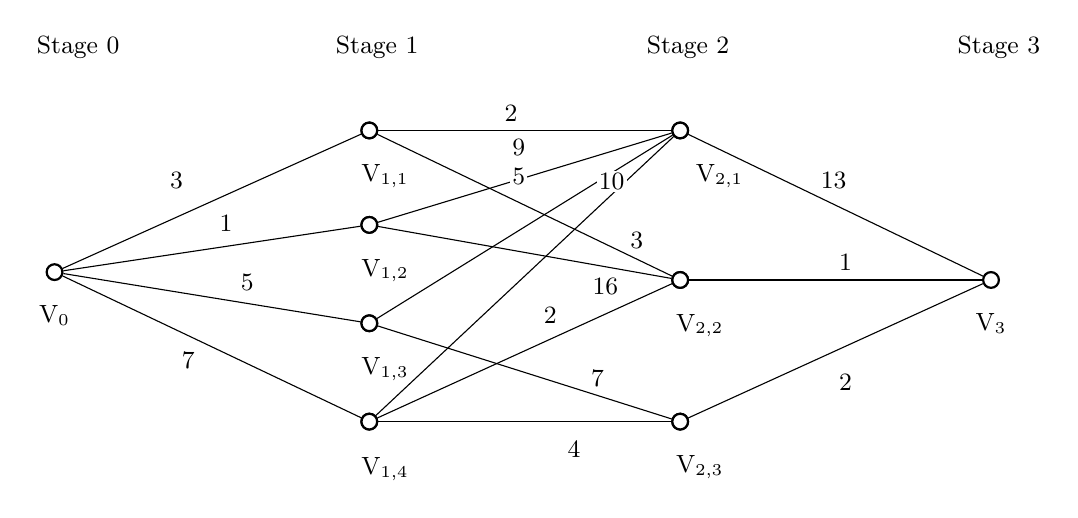
\begin{tikzpicture}[x=0.01cm,y=-0.01cm,v/.style={circle,draw,thick,fill=white,minimum size=2mm,inner sep=0pt},w/.style={font=\small,inner sep=0.8pt,fill=white},every node/.style={font=\small}]
\node[v] (v0) at (100,330) {};
\foreach \i/\y in {1/150,2/270,3/395,4/520} \node[v] (a\i) at (500,\y) {};
\foreach \i/\y in {1/150,2/340,3/520} \node[v] (b\i) at (895,\y) {};
\node[v] (v3) at (1290,340) {};
\foreach \i in {1,2,3,4} \draw (v0)--(a\i);
\foreach \a/\b in {a1/b1,a1/b2,a2/b1,a2/b2,a3/b1,a3/b3,a4/b1,a4/b2,a4/b3} \draw (\a)--(\b);
\foreach \i in {1,2,3} \draw (b\i)--(v3);
\foreach \i in {1,2,3,4} \node[v] at (a\i) {};
\foreach \i in {1,2,3} \node[v] at (b\i) {};
\node at (130,45) {Stage 0}; \node at (510,45) {Stage 1}; \node at (905,45) {Stage 2}; \node at (1300,45) {Stage 3};
\node at (100,385) {V$_0$}; \node at (520,208) {V$_{1,1}$}; \node at (520,328) {V$_{1,2}$}; \node at (520,453) {V$_{1,3}$}; \node at (520,580) {V$_{1,4}$};
\node at (945,208) {V$_{2,1}$}; \node at (920,398) {V$_{2,2}$}; \node at (920,578) {V$_{2,3}$}; \node at (1290,395) {V$_3$};
\node[w] at (255,213) {3}; \node[w] at (318,268) {1}; \node[w] at (345,343) {5}; \node[w] at (270,442) {7};
\node[w] at (680,128) {2}; \node[w] at (690,172) {9}; \node[w] at (690,208) {5}; \node[w] at (808,215) {10};
\node[w] at (840,290) {3}; \node[w] at (800,348) {16}; \node[w] at (730,385) {2}; \node[w] at (790,465) {7}; \node[w] at (760,555) {4};
\node[w] at (1090,213) {13}; \node[w] at (1105,318) {1}; \node[w] at (1105,470) {2};
\end{tikzpicture}
\end{center}
\begin{enumerate}[label=(\alph*)]
\item To find the shortest path (i.e., path with minimum weight) from V$_0$ to V$_3$ correctly, greedy
algorithm is applicable.
\item Following the same task as (a), dynamic programming is applicable.
\item From the stage perspective, the problem of finding the shortest path between the 4 stages shows
optimal substructure.
\item The path from V$_0$ to V$_3$ has minimum weight 7.
\item The path from V$_0$ to V$_3$ has minimum weight 6.
\end{enumerate}
\end{pastexam}

\begin{pastsoln}
答案：(b)(c)(d)。

這是多階段圖（multistage graph）：邊只從第 $k$ 階段連到第 $k + 1$ 階段，路徑依階段往右走。 原卷的圖在
選項右邊，這裡排在上面。 從圖讀出的邊權：
\begin{center}
\small
\begin{tabular}{ll}
\toprule
階段 & 邊（權重） \\
\midrule
$0 \to 1$ & $V_0V_{1,1}$ (3)，$V_0V_{1,2}$ (1)，$V_0V_{1,3}$ (5)，$V_0V_{1,4}$ (7) \\
$1 \to 2$ & $V_{1,1}V_{2,1}$ (2)，$V_{1,1}V_{2,2}$ (3)，$V_{1,2}V_{2,1}$ (9)，$V_{1,2}V_{2,2}$ (16)，
$V_{1,3}V_{2,1}$ (5)， \\
& $V_{1,3}V_{2,3}$ (7)，$V_{1,4}V_{2,1}$ (10)，$V_{1,4}V_{2,2}$ (2)，$V_{1,4}V_{2,3}$ (4) \\
$2 \to 3$ & $V_{2,1}V_3$ (13)，$V_{2,2}V_3$ (1)，$V_{2,3}V_3$ (2) \\
\bottomrule
\end{tabular}
\end{center}

\textbf{動態規劃}。 令 $d(v)$ 為 $V_0$ 到 $v$ 的最短距離，依階段往右算，每個點只看前一階段連過來的點
（資結書第~25.5~節 DAG 最短路徑的做法，也就是第~18~章的動態規劃）：
\begin{itemize}
\item 第 $1$ 階段：$d(V_{1,1}) = 3$，$d(V_{1,2}) = 1$，$d(V_{1,3}) = 5$，$d(V_{1,4}) = 7$。
\item 第 $2$ 階段：
$d(V_{2,1}) = \min(3 + 2,\ 1 + 9,\ 5 + 5,\ 7 + 10) = 5$；
$d(V_{2,2}) = \min(3 + 3,\ 1 + 16,\ 7 + 2) = 6$；
$d(V_{2,3}) = \min(5 + 7,\ 7 + 4) = 11$。
\item 第 $3$ 階段：$d(V_3) = \min(5 + 13,\ 6 + 1,\ 11 + 2) = 7$。
\end{itemize}
最短路徑 $V_0 \to V_{1,1} \to V_{2,2} \to V_3$，權重 $3 + 3 + 1 = 7$。

\textbf{逐項}：
\begin{itemize}
\item (a) 錯。 貪心法每一步走目前最輕的邊：$V_0 \to V_{1,2}$ (1)，$V_{1,2}$ 出去最輕的是 $V_{2,1}$ (9)，
再到 $V_3$ (13)，共 $23$，遠大於 $7$。 第一步看起來最划算的 $V_{1,2}$，後面的邊都很重。
\item (b) 對。 上面的計算就是動態規劃，答案正確。
\item (c) 對。 最短路徑有最佳子結構：$V_0$ 到 $V_3$ 的最短路徑經過 $V_{2,2}$ 時，它的前段一定是 $V_0$ 到
$V_{2,2}$ 的最短路徑（否則換成更短的前段，整條更短）。 多階段的動態規劃正是靠這個性質，一階段一階段算。
\item (d) 對。 最短是 $7$。
\item (e) 錯。 $6$ 是 $V_0$ 到 $V_{2,2}$ 的距離，不是到 $V_3$。
\end{itemize}
\end{pastsoln}
